\documentclass[11pt,a4paper]{article}
\usepackage[margin=2.2cm]{geometry}
\usepackage{verbatim,booktabs,graphicx,amsmath,xcolor,float,caption}
\usepackage[T1]{fontenc}
\usepackage{lmodern}
\graphicspath{{fig/}}
\newcommand{\DataState}{final, 2026-11-27 13:04}
\newcommand{\DataNote}{\textbf{Final.} All 60 runs finished (2026-11-27 13:04).}
   % defines \DataState and \DataNote (written by prelim.sh)
\title{ALF node throughput: GPU node vs CPU node\\\large SuperMUC-NG Phase 2, test of 2026-11-27 and 28}
\author{}
\date{\DataState}
\begin{document}
\maketitle
\begin{center}\fcolorbox{red}{white}{\parbox{0.9\textwidth}{\DataNote}}\end{center}

\section{What is compared}
One full Phase 2 node per simulation: either its two CPUs alone (112 cores, build \texttt{build\_cpu-pp}, ALF 410c7b04)
or its four Intel Data Center GPU Max 1550 (8 tiles) with ALF 410c7b04 (\texttt{build\_pp}) and with the Intel-optimised
production binary (branch intel-batched, d1060305, run-time switches of the production run RUN\_L36\_batched).
Hubbard model, square lattice, $L\in\{16,24,32,36,40,44,48,52,56\}$, $\beta=4$, $\Delta\tau=0.1$, $h_0=0$, $U=5.25$, $M_z=$ F,
Symm and Checkerboard on, Ltau $=0$, submatrix updates with $N_\text{delay}=64$, Nwrap $=10$.
Each run does NBin sweeps (NSweep $=1$); the first is dropped, the others are timed one by one: NBin $=11$ (10 timed sweeps) for the final runs of every GPU configuration at $\beta=4$, 4 to 6 (3 to 5 timed) for the scan runs of the tuning, 3 to 4 (2 to 3 timed) at $\beta=L$. The CPU node was measured up to $L=40$ (\texttt{t1}, 5 timed sweeps) at $\beta=4$ and up to $L=36$ at $\beta=L$; above that only the GPU node was run.
Both GPU codes include the fix for the NaN determinant phase (commit 0b3ffba4; the raw LU product underflows from $L\approx54$): Intel-optimised \texttt{intel-batched-detfix} 65800b82 (= d1060305 + fix), ALF GPU \texttt{antrag/2026-11-27-detfix} 90a51fcb (= 410c7b04 + fix). Check at $L=56$: acceptance 0.328 for both codes (0.27 and NaN observables without the fix); $L=24$ reproduces the earlier output (acceptance 0.332416942866162).
All walkers of a run form one parameter set; one bin is the average of one sweep over all walkers.
All walkers of a run form one parameter set; one bin is the average of one sweep over all walkers.

\section{Node and layouts (x axes of the figures)}
Node: 2 sockets $\times$ 56 cores (Xeon Platinum 8480L), 2 NUMA domains (cores 0--55 and 56--111). GPUs 0, 1 are
attached to NUMA domain 0, GPUs 2, 3 to NUMA domain 1, so each tile has 14 nearby cores. No rank crosses a NUMA domain.

\begin{table}[H]\centering\small
\caption{CPU layouts. Tag \texttt{t}$T$ = $T$ OpenMP threads per MPI rank (one walker per rank), ranks split evenly over
the two sockets, each rank pinned to $T$ consecutive physical cores of one socket.}
\begin{tabular}{@{}llrrrr@{}}\toprule
tag & commit & threads per rank & ranks (walkers) & ranks per socket & cores used\\\midrule
\texttt{t1} & \texttt{410c7b04} & 1 & 112 & 56 & 112\\
\texttt{t2} & \texttt{410c7b04} & 2 & 56 & 28 & 112\\
\texttt{t4} & \texttt{410c7b04} & 4 & 28 & 14 & 112\\
\texttt{t6} & \texttt{410c7b04} & 6 & 18 & 9 & 108\\
\texttt{t8} & \texttt{410c7b04} & 8 & 14 & 7 & 112\\\bottomrule
\end{tabular}\end{table}

\begin{table}[H]\centering\small
\caption{GPU layouts (both GPU binaries). Tag \texttt{w}$W$\texttt{t}$T$ = $W$ walkers (MPI ranks) per tile on all 8 tiles,
$T$ OpenMP host threads per rank. The $W$ ranks of a tile get disjoint core slices of $\lfloor14/W\rfloor$ cores (plus hyperthreads); compute engines per tile
$\min(W,4)$ (\texttt{ZEX\_NUMBER\_OF\_CCS}). \texttt{w4t3} is the production layout.}
\begin{tabular}{@{}lrrrr@{}}\toprule
tag & walkers per tile & ranks (walkers) & threads per rank & cores per rank\\\midrule
\texttt{w2t7} & 2 & 16 & 7 & 7\\
\texttt{w4t1}, \texttt{w4t2}, \texttt{w4t3} & 4 & 32 & 1, 2, 3 & 3\\
\texttt{w6t2} & 6 & 48 & 2 & 2\\
\texttt{w7t2} & 7 & 56 & 2 & 2\\
\texttt{w8t1} & 8 & 64 & 1 & 1\\\bottomrule
\end{tabular}\end{table}

\section{Parameters}
\subsection*{ALF parameter file}
Generated by \texttt{make\_params.py} from the production file of RUN\_L24 (jakob\_params), one parameter set per run
(\texttt{mpi\_per\_parameter\_set} = number of MPI ranks of the node; no tempering exchange). Example: $L=40$, $\beta=4$, 56 ranks.
\begin{table}[H]\centering\small
\caption{Parameters that differ between runs; everything else is fixed as in the listing below.}
\begin{tabular}{@{}lll@{}}\toprule
parameter & value & note\\\midrule
\texttt{L1}, \texttt{L2} & $L$ & 16, 24, 32, 36, 40, 44, 48, 52, 56\\
\texttt{N\_Phi} & $L^2/2$ & flux, as in the production runs\\
\texttt{Beta} & 4 & \texttt{Dtau} $=0.1$, so 40 time slices at $\beta=4$, $10L$ at $\beta=L$\\
\texttt{Ltau} & 0 & no time-displaced measurements\\
\texttt{ham\_h0}, \texttt{ham\_U} & 0, 5.25 & no defect, one $U$\\
\texttt{NSweep}, \texttt{NBin} & 1, 3 to 11 & one sweep per bin, so every sweep is timed\\
\texttt{CPU\_MAX} & 0 & run ends after NBin bins\\
\texttt{mpi\_per\_parameter\_set} & ranks & 8 to 112\\
\texttt{N\_delay} & 64, tuned & 64 to 1024, see the tuning section\\\bottomrule
\end{tabular}\end{table}
Fixed (asserted by the script): \texttt{Mz}~$=$~.F., \texttt{Symm} and \texttt{Checkerboard} .T., \texttt{N\_FL}~$=2$, \texttt{N\_SUN}~$=2$,
\texttt{Sequential\_scheme} ``submatrix'', \texttt{Nwrap}~$=10$, \texttt{Propose\_S0}, \texttt{Global\_moves}, \texttt{Langevin}, \texttt{HMC} all .F.
\small\verbatiminput{params_example.txt}\normalsize

\subsection*{Run environment}
\begin{itemize}\itemsep0pt
\item Builds (ALF commit 410c7b04 with the fix 0b3ffba4 for the GPU codes): \texttt{configure.sh IntelLLVM PP GPU=intel HDF5} (GPU) and \texttt{IntelLLVM PP HDF5} (CPU), i.e. \texttt{-DMPI -DTEMPERING -DPARALLEL\_PARAMS -DHDF5}; Intel oneAPI 2025.3, Intel MPI 2021.15, oneMKL 2025.3, LRZ HDF5.
\item Launch: one \texttt{srun} step per node (\texttt{-N1 -n1 -c 224 --cpu-bind=none --mem=0 --exclusive}), \texttt{mpiexec -bootstrap fork -n} NR \texttt{-ppn} NR \texttt{pin.sh ALF.out}; \texttt{I\_MPI\_PIN=0}, \texttt{OMP\_PROC\_BIND=close}, \texttt{OMP\_PLACES=cores}, \texttt{OMP\_NUM\_THREADS=MKL\_NUM\_THREADS=}$T$.
\item Pinning (\texttt{pin.sh}): CPU: $T$ consecutive physical cores per rank inside one socket (\texttt{numactl --physcpubind --membind}). GPU: \texttt{ZE\_AFFINITY\_MASK}~$=$ tile of the rank, the $W$ ranks of a tile get disjoint slices of $\lfloor14/W\rfloor$ cores plus their hyperthreads, memory bound to the socket of the tile.
\item GPU runs: \texttt{OMP\_TARGET\_OFFLOAD=MANDATORY}, \texttt{ZE\_FLAT\_DEVICE\_HIERARCHY=FLAT}, \texttt{ZEX\_NUMBER\_OF\_CCS} $=\min(W,4)$ per tile, \texttt{ALF\_UNSTABLE\_THRESHOLD=1e-4}.
\item Intel-optimised code, production switches (not tuned further: no effect beyond noise): \texttt{LIBOMPTARGET\_LEVEL\_ZERO\_STAGING\_BUFFER\_SIZE=1048576}, \texttt{ALFSH\_ASYNCBLK=1}, \texttt{ALFSH\_DEVQR=2}, \texttt{ALFSH\_DEVUNMQR=1}, \texttt{ALFSH\_QRNB=16}, \texttt{ALFSH\_OBSCORR=1}, \texttt{ALFSH\_BLKFUSE=5}, \texttt{ALFSH\_BLKPF=1}; \texttt{LD\_LIBRARY\_PATH} to the directory with \texttt{libalfsb.so}, \texttt{libalfdevqr.so}.
\item Seeds: \texttt{random.seed(1000+$L$)}, one 30-bit integer per rank (same for every layout of an $L$).
\item Scanned in the tuning (ranges): layout $W\times T$ in \{2$\times$7, 4$\times$1, 4$\times$2, 4$\times$3, 6$\times$2, 7$\times$2, 8$\times$1\}; \texttt{N\_delay} $\in\{64,128,256,512,1024\}$; Intel-optimised only \texttt{ALFSH\_ASYNCBLK} $\in\{1,0\}$, \texttt{ALFSH\_BLKFUSE} $\in\{3,5,8\}$, \texttt{ALFSH\_QRNB} $\in\{8,16,32,64\}$ (defaults in bold in the code: 1, 5, 16, 64). Earlier tests without effect: \texttt{ALF\_GPU\_TL} $\in\{1,2,4\}$, \texttt{TR} $\in\{1,2,4\}$, \texttt{VB} $\in\{4,8,16\}$, \texttt{ALFSH\_BLKPF}~0/1. Not varied: \texttt{Nwrap}.
\end{itemize}

\section{Tuning of the GPU node}
\textbf{Pinning.} In the first series (\texttt{w}$W$\texttt{t}$T$ layouts with $W\ge2$) all $W$ processes of a tile were pinned to the same 14 cores; with OpenMP places = cores the first threads of these processes then share cores. Measured effect (Intel-optimised, $\beta=4$): $L=40$, 4$\times$1: 38\,s $\to$ 16.9\,s per sweep; ALF GPU, $L=32$, $\beta=L$, 4$\times$3: 88.3\,s $\to$ 46.7\,s (the production run of 11 November had 51.9\,s). All GPU results of this report use disjoint core slices: the $W$ processes of a tile get $\lfloor14/W\rfloor$ cores each (plus their hyperthreads).

\textbf{Search} (\texttt{tune.py}, one full node per run). For every code and every $L$: (A) layouts 2$\times$7, 4$\times$1, 4$\times$2, 4$\times$3, 6$\times$2, 7$\times$2, 8$\times$1 (processes per tile $\times$ threads); (B) from the best layout one parameter group at a time: $N_\text{delay}\in\{128,256,512,1024\}$ (default 64), and for the Intel-optimised code \texttt{ASYNCBLK}$=0$, \texttt{BLKFUSE}$\in\{3,8\}$, \texttt{QRNB}$\in\{8,32,64\}$; (C) the groups that gained at least 3\,\% combined, plus a repeat of the baseline; (F) the two best configurations rerun with 10 timed sweeps, the faster one is the result. $\beta=L$ uses the settings found at $\beta=4$; if a layout runs out of device memory (more walkers need more memory at 10$L$ time slices) the next layout is tried (down to 1 process per tile). Tested before the search and without effect beyond the noise of 1 to 3\,\%: \texttt{ALF\_GPU\_TL}, \texttt{TR}, \texttt{VB}, \texttt{BLKPF}.

\textbf{Result.} Up to $L\approx 40$ only the layout matters ($N_\text{delay}=64$ stays best, larger values lose up to 40\,\% at $L=24$); from $L\approx 44$ $N_\text{delay}=256$ gains 3 to 14\,\%, at $L=56$ 256 or 512 are best. Larger systems need more walkers per tile at $\beta=4$ (7 to 8) than small ones (4).

\begin{table}[H]\centering\small
\caption{Tuned settings per code and $L$ (best of the search; $N_\text{delay}=64$ and the production switches where not stated).}
\newcommand{\TunedTable}{%
\begin{tabular}{rllll}
$L$ & code & layout $\beta=4$ & settings $\beta=4$ & layout $\beta=L$\\
\hline
16 & ALF GPU Intel-opt. & 4 proc./tile $\times$ 1 thr. & default & 4 proc./tile $\times$ 1 thr.\\
16 & ALF GPU & 4 proc./tile $\times$ 2 thr. & default & 4 proc./tile $\times$ 2 thr.\\
\hline
24 & ALF GPU Intel-opt. & 4 proc./tile $\times$ 3 thr. & default & 4 proc./tile $\times$ 3 thr.\\
24 & ALF GPU & 4 proc./tile $\times$ 2 thr. & default & 4 proc./tile $\times$ 2 thr.\\
\hline
32 & ALF GPU Intel-opt. & 4 proc./tile $\times$ 3 thr. & default & 4 proc./tile $\times$ 3 thr.\\
32 & ALF GPU & 4 proc./tile $\times$ 3 thr. & default & 4 proc./tile $\times$ 3 thr.\\
\hline
36 & ALF GPU Intel-opt. & 4 proc./tile $\times$ 3 thr. & default & 4 proc./tile $\times$ 3 thr.\\
36 & ALF GPU & 4 proc./tile $\times$ 3 thr. & default & 4 proc./tile $\times$ 3 thr.\\
\hline
40 & ALF GPU Intel-opt. & 7 proc./tile $\times$ 2 thr. & default & 7 proc./tile $\times$ 2 thr.\\
40 & ALF GPU & 7 proc./tile $\times$ 2 thr. & $N\_\text{delay}=$256 & 7 proc./tile $\times$ 2 thr.\\
\hline
44 & ALF GPU Intel-opt. & 7 proc./tile $\times$ 2 thr. & default & 4 proc./tile $\times$ 3 thr.\\
44 & ALF GPU & 7 proc./tile $\times$ 2 thr. & $N\_\text{delay}=$256 & 4 proc./tile $\times$ 3 thr.\\
\hline
48 & ALF GPU Intel-opt. & 7 proc./tile $\times$ 2 thr. & default & 2 proc./tile $\times$ 7 thr.\\
48 & ALF GPU & 7 proc./tile $\times$ 2 thr. & $N\_\text{delay}=$256 & 2 proc./tile $\times$ 7 thr.\\
\hline
52 & ALF GPU Intel-opt. & 7 proc./tile $\times$ 2 thr. & $N\_\text{delay}=$256 & 2 proc./tile $\times$ 7 thr.\\
52 & ALF GPU & 8 proc./tile $\times$ 1 thr. & $N\_\text{delay}=$256 & 2 proc./tile $\times$ 7 thr.\\
\hline
56 & ALF GPU Intel-opt. & 7 proc./tile $\times$ 2 thr. & $N\_\text{delay}=$256 & 1 proc./tile $\times$ 14 thr.\\
56 & ALF GPU & 7 proc./tile $\times$ 2 thr. & $N\_\text{delay}=$512 & 1 proc./tile $\times$ 14 thr.\\
\hline
\end{tabular}}

\TunedTable
\end{table}

\section{Timing and throughput}
Rank 0 writes one bin per sweep to \texttt{data.h5}, one HDF5 write per observable. The modification time of the file is
logged with ns resolution; the writes form 12 bursts (file creation + 11 bins). For the timed sweeps $k=2,\dots,11$:
\[
t_\text{comp}(k)=\text{first write of bin }k-\text{last write of bin }k{-}1,\qquad
t_\text{io}(k)=\text{last write of bin }k-\text{first write of bin }k .
\]
Production writes one bin per 10 sweeps, so the cost per sweep is $t_\text{sweep}=t_\text{comp}+t_\text{io}/10$.
Walkers synchronise at every bin, so $t_\text{sweep}$ is the time of the slowest walker. With $N_w$ walkers on the node,
\[
\text{throughput}=\frac{3600\,N_w}{\bar t_\text{sweep}}\ \text{sweeps per node-hour},\qquad
\sigma=\text{throughput}\cdot\frac{\sigma_{\bar t}}{\bar t},
\]
with $\sigma_{\bar t}$ the standard error of the 10 sweep times. Each configuration was run once.

Energy per sweep (estimate from vendor TDP, to be checked): CPU-only node $2\times350$\,W $=700$\,W,
GPU node $4\times600$\,W $+700$\,W $=3100$\,W; $E=P_\text{node}\cdot3600/\text{throughput}$.

\section{Results}
\begin{table}[h]\centering\small
\caption{Best layout per side: node throughput (sweeps per node-hour) and factor against the best CPU layout.}\label{tab:summary}
\begin{tabular}{@{}rllllr@{}}\toprule
$L$ & side & commit & best layout & sweeps per node-hour & factor vs CPU\\\midrule
16 & CPU & \texttt{410c7b04} & \texttt{t1} & $144\,581 \pm 780$ & 1.00\\
16 & GPU & \texttt{410c7b04} & \texttt{w4t2\_F0} & $189\,332 \pm 1\,205$ & 1.31\\
16 & GPU Intel-opt. & \texttt{d1060305} & \texttt{w4t1\_F0} & $391\,560 \pm 3\,065$ & 2.71\\
\addlinespace
24 & CPU & \texttt{410c7b04} & \texttt{t1} & $18\,266 \pm 8$ & 1.00\\
24 & GPU & \texttt{410c7b04} & \texttt{w4t2\_F0} & $53\,545 \pm 152$ & 2.93\\
24 & GPU Intel-opt. & \texttt{d1060305} & \texttt{w4t3\_F0} & $105\,468 \pm 141$ & 5.77\\
\addlinespace
32 & CPU & \texttt{410c7b04} & \texttt{t1} & $2\,475 \pm 0$ & 1.00\\
32 & GPU & \texttt{410c7b04} & \texttt{w4t3\_F0} & $19\,411 \pm 14$ & 7.84\\
32 & GPU Intel-opt. & \texttt{d1060305} & \texttt{w4t3\_F0} & $29\,338 \pm 36$ & 11.86\\
\addlinespace
36 & CPU & \texttt{410c7b04} & \texttt{t1} & $1\,728 \pm 1$ & 1.00\\
36 & GPU & \texttt{410c7b04} & \texttt{w4t3\_F0} & $11\,372 \pm 7$ & 6.58\\
36 & GPU Intel-opt. & \texttt{d1060305} & \texttt{w4t3\_F0} & $15\,636 \pm 6$ & 9.05\\
\addlinespace
40 & CPU & \texttt{410c7b04} & \texttt{t1} & $933 \pm 0$ & 1.00\\
40 & GPU & \texttt{410c7b04} & \texttt{w7t2\_F0} & $7\,524 \pm 12$ & 8.06\\
40 & GPU Intel-opt. & \texttt{d1060305} & \texttt{w7t2\_F0} & $8\,899 \pm 12$ & 9.54\\
\addlinespace
44 & CPU & \texttt{410c7b04} & -- & running & --\\
44 & GPU & \texttt{410c7b04} & \texttt{w7t2\_F0} & $5\,459 \pm 5$ & --\\
44 & GPU Intel-opt. & \texttt{d1060305} & \texttt{w7t2\_F0} & $5\,304 \pm 13$ & --\\
\addlinespace
48 & CPU & \texttt{410c7b04} & -- & running & --\\
48 & GPU & \texttt{410c7b04} & \texttt{w7t2\_F0} & $3\,578 \pm 2$ & --\\
48 & GPU Intel-opt. & \texttt{d1060305} & \texttt{w7t2\_F0} & $3\,588 \pm 3$ & --\\
\addlinespace
52 & CPU & \texttt{410c7b04} & -- & running & --\\
52 & GPU & \texttt{410c7b04} & \texttt{w8t1\_F0} & $2\,288 \pm 2$ & --\\
52 & GPU Intel-opt. & \texttt{d1060305} & \texttt{w7t2\_F0} & $2\,345 \pm 1$ & --\\
\addlinespace
56 & CPU & \texttt{410c7b04} & -- & running & --\\
56 & GPU & \texttt{410c7b04} & \texttt{w7t2\_F0} & $1\,684 \pm 1$ & --\\
56 & GPU Intel-opt. & \texttt{d1060305} & \texttt{w7t2\_F0} & $1\,667 \pm 1$ & --\\
\bottomrule\end{tabular}\end{table}
\begin{table}[h]\centering\small
\caption{All layouts at $L=16$ ($\beta=4$). Time per sweep of one walker (mean of the timed sweeps, $\pm$ standard error; averaged over repeats) and node throughput.}
\begin{tabular}{@{}llllrr@{}}\toprule
side & commit & tag & layout & time per sweep (s) & sweeps per node-hour\\\midrule
CPU & \texttt{410c7b04} & \texttt{t1} & 112 ranks $\times$ 1 thr. & $2.789 \pm 0.015$ & $144\,581 \pm 780$\\
CPU & \texttt{410c7b04} & \texttt{t2} & 56 ranks $\times$ 2 thr. & $2.384 \pm 0.008$ & $84\,566 \pm 287$\\
CPU & \texttt{410c7b04} & \texttt{t4} & 28 ranks $\times$ 4 thr. & $2.115 \pm 0.006$ & $47\,660 \pm 146$\\
CPU & \texttt{410c7b04} & \texttt{t6} & 18 ranks $\times$ 6 thr. & $1.982 \pm 0.001$ & $32\,685 \pm 20$\\
CPU & \texttt{410c7b04} & \texttt{t8} & 14 ranks $\times$ 8 thr. & $1.961 \pm 0.001$ & $25\,700 \pm 18$\\
GPU & \texttt{410c7b04} & \texttt{w1t14} & 1 walker/tile, 14 thr. & $0.435 \pm 0.004$ & $66\,272 \pm 634$\\
GPU & \texttt{410c7b04} & \texttt{w4t2\_F0} & 4 walker/tile, 2 thr. & $0.609 \pm 0.004$ & $189\,332 \pm 1\,205$\\
GPU Intel-opt. & \texttt{d1060305} & \texttt{w1t14} & 1 walker/tile, 14 thr. & $0.261 \pm 0.003$ & $110\,529 \pm 1\,168$\\
GPU Intel-opt. & \texttt{d1060305} & \texttt{w4t1\_F0} & 4 walker/tile, 1 thr. & $0.294 \pm 0.002$ & $391\,560 \pm 3\,065$\\
\bottomrule\end{tabular}\end{table}
\begin{table}[h]\centering\small
\caption{All layouts at $L=24$ ($\beta=4$). Time per sweep of one walker (mean of the timed sweeps, $\pm$ standard error; averaged over repeats) and node throughput.}
\begin{tabular}{@{}llllrr@{}}\toprule
side & commit & tag & layout & time per sweep (s) & sweeps per node-hour\\\midrule
CPU & \texttt{410c7b04} & \texttt{t1} & 112 ranks $\times$ 1 thr. & $22.074 \pm 0.010$ & $18\,266 \pm 8$\\
CPU & \texttt{410c7b04} & \texttt{t2} & 56 ranks $\times$ 2 thr. & $13.246 \pm 0.005$ & $15\,220 \pm 6$\\
CPU & \texttt{410c7b04} & \texttt{t4} & 28 ranks $\times$ 4 thr. & $10.107 \pm 0.007$ & $9\,973 \pm 7$\\
CPU & \texttt{410c7b04} & \texttt{t6} & 18 ranks $\times$ 6 thr. & $9.099 \pm 0.009$ & $7\,122 \pm 7$\\
CPU & \texttt{410c7b04} & \texttt{t8} & 14 ranks $\times$ 8 thr. & $8.735 \pm 0.005$ & $5\,770 \pm 3$\\
GPU & \texttt{410c7b04} & \texttt{w1t14} & 1 walker/tile, 14 thr. & $1.298 \pm 0.002$ & $22\,181 \pm 31$\\
GPU & \texttt{410c7b04} & \texttt{w4t2\_F0} & 4 walker/tile, 2 thr. & $2.151 \pm 0.006$ & $53\,545 \pm 152$\\
GPU Intel-opt. & \texttt{d1060305} & \texttt{w1t14} & 1 walker/tile, 14 thr. & $0.569 \pm 0.001$ & $50\,607 \pm 99$\\
GPU Intel-opt. & \texttt{d1060305} & \texttt{w4t3\_F0} & 4 walker/tile, 3 thr. & $1.092 \pm 0.002$ & $105\,468 \pm 141$\\
\bottomrule\end{tabular}\end{table}
\begin{table}[h]\centering\small
\caption{All layouts at $L=32$ ($\beta=4$). Time per sweep of one walker (mean of the timed sweeps, $\pm$ standard error; averaged over repeats) and node throughput.}
\begin{tabular}{@{}llllrr@{}}\toprule
side & commit & tag & layout & time per sweep (s) & sweeps per node-hour\\\midrule
CPU & \texttt{410c7b04} & \texttt{t1} & 112 ranks $\times$ 1 thr. & $162.937 \pm 0.028$ & $2\,475 \pm 0$\\
CPU & \texttt{410c7b04} & \texttt{t2} & 56 ranks $\times$ 2 thr. & $95.704 \pm 0.021$ & $2\,106 \pm 0$\\
CPU & \texttt{410c7b04} & \texttt{t4} & 28 ranks $\times$ 4 thr. & $69.022 \pm 0.019$ & $1\,460 \pm 0$\\
CPU & \texttt{410c7b04} & \texttt{t6} & 18 ranks $\times$ 6 thr. & $54.431 \pm 0.026$ & $1\,190 \pm 1$\\
CPU & \texttt{410c7b04} & \texttt{t8} & 14 ranks $\times$ 8 thr. & $50.380 \pm 0.012$ & $1\,000 \pm 0$\\
GPU & \texttt{410c7b04} & \texttt{w1t14} & 1 walker/tile, 14 thr. & $3.082 \pm 0.004$ & $9\,346 \pm 11$\\
GPU & \texttt{410c7b04} & \texttt{w4t3\_F0} & 4 walker/tile, 3 thr. & $5.935 \pm 0.004$ & $19\,411 \pm 14$\\
GPU Intel-opt. & \texttt{d1060305} & \texttt{w1t14} & 1 walker/tile, 14 thr. & $1.423 \pm 0.001$ & $20\,234 \pm 18$\\
GPU Intel-opt. & \texttt{d1060305} & \texttt{w4t3\_F0} & 4 walker/tile, 3 thr. & $3.927 \pm 0.005$ & $29\,338 \pm 36$\\
\bottomrule\end{tabular}\end{table}
\begin{table}[h]\centering\small
\caption{All layouts at $L=36$ ($\beta=4$). Time per sweep of one walker (mean of the timed sweeps, $\pm$ standard error; averaged over repeats) and node throughput.}
\begin{tabular}{@{}llllrr@{}}\toprule
side & commit & tag & layout & time per sweep (s) & sweeps per node-hour\\\midrule
CPU & \texttt{410c7b04} & \texttt{t1} & 112 ranks $\times$ 1 thr. & $233.296 \pm 0.081$ & $1\,728 \pm 1$\\
CPU & \texttt{410c7b04} & \texttt{t2} & 56 ranks $\times$ 2 thr. & $124.077 \pm 0.058$ & $1\,625 \pm 1$\\
CPU & \texttt{410c7b04} & \texttt{t4} & 28 ranks $\times$ 4 thr. & $77.811 \pm 0.034$ & $1\,295 \pm 1$\\
CPU & \texttt{410c7b04} & \texttt{t6} & 18 ranks $\times$ 6 thr. & $63.220 \pm 0.058$ & $1\,025 \pm 1$\\
CPU & \texttt{410c7b04} & \texttt{t8} & 14 ranks $\times$ 8 thr. & $55.436 \pm 0.034$ & $909 \pm 1$\\
GPU & \texttt{410c7b04} & \texttt{w1t14} & 1 walker/tile, 14 thr. & $4.780 \pm 0.005$ & $6\,025 \pm 6$\\
GPU & \texttt{410c7b04} & \texttt{w4t3\_F0} & 4 walker/tile, 3 thr. & $10.130 \pm 0.006$ & $11\,372 \pm 7$\\
GPU Intel-opt. & \texttt{d1060305} & \texttt{w1t14} & 1 walker/tile, 14 thr. & $2.489 \pm 0.002$ & $11\,570 \pm 9$\\
GPU Intel-opt. & \texttt{d1060305} & \texttt{w4t3\_F0} & 4 walker/tile, 3 thr. & $7.367 \pm 0.003$ & $15\,636 \pm 6$\\
\bottomrule\end{tabular}\end{table}
\begin{table}[h]\centering\small
\caption{All layouts at $L=40$ ($\beta=4$). Time per sweep of one walker (mean of the timed sweeps, $\pm$ standard error; averaged over repeats) and node throughput.}
\begin{tabular}{@{}llllrr@{}}\toprule
side & commit & tag & layout & time per sweep (s) & sweeps per node-hour\\\midrule
CPU & \texttt{410c7b04} & \texttt{t1} & 112 ranks $\times$ 1 thr. & $432.159 \pm 0.236$ & $933 \pm 0$\\
GPU & \texttt{410c7b04} & \texttt{w7t2\_F0} & 7 walker/tile, 2 thr. & $26.793 \pm 0.043$ & $7\,524 \pm 12$\\
GPU & \texttt{410c7b04} & \texttt{w7t2\_F1} & 7 walker/tile, 2 thr. & $27.777 \pm 0.056$ & $7\,258 \pm 15$\\
GPU Intel-opt. & \texttt{d1060305} & \texttt{w1t14} & 1 walker/tile, 14 thr. & $4.861 \pm 0.004$ & $5\,924 \pm 5$\\
GPU Intel-opt. & \texttt{d1060305} & \texttt{w7t2\_F0} & 7 walker/tile, 2 thr. & $22.653 \pm 0.030$ & $8\,899 \pm 12$\\
\bottomrule\end{tabular}\end{table}
\begin{table}[h]\centering\small
\caption{All layouts at $L=44$ ($\beta=4$). Time per sweep of one walker (mean of the timed sweeps, $\pm$ standard error; averaged over repeats) and node throughput.}
\begin{tabular}{@{}llllrr@{}}\toprule
side & commit & tag & layout & time per sweep (s) & sweeps per node-hour\\\midrule
GPU & \texttt{410c7b04} & \texttt{w1t14} & 1 walker/tile, 14 thr. & $9.556 \pm 0.010$ & $3\,014 \pm 3$\\
GPU & \texttt{410c7b04} & \texttt{w7t2\_F0} & 7 walker/tile, 2 thr. & $36.930 \pm 0.032$ & $5\,459 \pm 5$\\
GPU & \texttt{410c7b04} & \texttt{w7t2\_F1} & 7 walker/tile, 2 thr. & $41.826 \pm 0.103$ & $4\,820 \pm 12$\\
GPU Intel-opt. & \texttt{d1060305} & \texttt{w1t14} & 1 walker/tile, 14 thr. & $7.248 \pm 0.009$ & $3\,973 \pm 5$\\
GPU Intel-opt. & \texttt{d1060305} & \texttt{w7t2\_F0} & 7 walker/tile, 2 thr. & $38.008 \pm 0.091$ & $5\,304 \pm 13$\\
\bottomrule\end{tabular}\end{table}
\begin{table}[h]\centering\small
\caption{All layouts at $L=48$ ($\beta=4$). Time per sweep of one walker (mean of the timed sweeps, $\pm$ standard error; averaged over repeats) and node throughput.}
\begin{tabular}{@{}llllrr@{}}\toprule
side & commit & tag & layout & time per sweep (s) & sweeps per node-hour\\\midrule
GPU & \texttt{410c7b04} & \texttt{w1t14} & 1 walker/tile, 14 thr. & $13.384 \pm 0.015$ & $2\,152 \pm 2$\\
GPU & \texttt{410c7b04} & \texttt{w7t2\_F0} & 7 walker/tile, 2 thr. & $56.346 \pm 0.035$ & $3\,578 \pm 2$\\
GPU & \texttt{410c7b04} & \texttt{w7t2\_F1} & 7 walker/tile, 2 thr. & $63.805 \pm 0.116$ & $3\,160 \pm 6$\\
GPU Intel-opt. & \texttt{d1060305} & \texttt{w1t14} & 1 walker/tile, 14 thr. & $10.561 \pm 0.010$ & $2\,727 \pm 3$\\
GPU Intel-opt. & \texttt{d1060305} & \texttt{w7t2\_F0} & 7 walker/tile, 2 thr. & $56.184 \pm 0.046$ & $3\,588 \pm 3$\\
\bottomrule\end{tabular}\end{table}
\begin{table}[h]\centering\small
\caption{All layouts at $L=52$ ($\beta=4$). Time per sweep of one walker (mean of the timed sweeps, $\pm$ standard error; averaged over repeats) and node throughput.}
\begin{tabular}{@{}llllrr@{}}\toprule
side & commit & tag & layout & time per sweep (s) & sweeps per node-hour\\\midrule
GPU & \texttt{410c7b04} & \texttt{w1t14} & 1 walker/tile, 14 thr. & $18.759 \pm 0.020$ & $1\,535 \pm 2$\\
GPU & \texttt{410c7b04} & \texttt{w8t1\_F0} & 8 walker/tile, 1 thr. & $100.687 \pm 0.087$ & $2\,288 \pm 2$\\
GPU & \texttt{410c7b04} & \texttt{w8t1\_F1} & 8 walker/tile, 1 thr. & $111.589 \pm 0.154$ & $2\,065 \pm 3$\\
GPU Intel-opt. & \texttt{d1060305} & \texttt{w1t14} & 1 walker/tile, 14 thr. & $15.974 \pm 0.018$ & $1\,803 \pm 2$\\
GPU Intel-opt. & \texttt{d1060305} & \texttt{w7t2\_F0} & 7 walker/tile, 2 thr. & $85.960 \pm 0.033$ & $2\,345 \pm 1$\\
GPU Intel-opt. & \texttt{d1060305} & \texttt{w7t2\_F1} & 7 walker/tile, 2 thr. & $91.570 \pm 0.051$ & $2\,202 \pm 1$\\
\bottomrule\end{tabular}\end{table}
\begin{table}[h]\centering\small
\caption{All layouts at $L=56$ ($\beta=4$). Time per sweep of one walker (mean of the timed sweeps, $\pm$ standard error; averaged over repeats) and node throughput.}
\begin{tabular}{@{}llllrr@{}}\toprule
side & commit & tag & layout & time per sweep (s) & sweeps per node-hour\\\midrule
GPU & \texttt{410c7b04} & \texttt{w1t14} & 1 walker/tile, 14 thr. & $25.779 \pm 0.025$ & $1\,117 \pm 1$\\
GPU & \texttt{410c7b04} & \texttt{w7t2\_F0} & 7 walker/tile, 2 thr. & $119.708 \pm 0.062$ & $1\,684 \pm 1$\\
GPU & \texttt{410c7b04} & \texttt{w7t2\_F1} & 7 walker/tile, 2 thr. & $136.773 \pm 0.192$ & $1\,474 \pm 2$\\
GPU Intel-opt. & \texttt{d1060305} & \texttt{w1t14} & 1 walker/tile, 14 thr. & $22.524 \pm 0.007$ & $1\,279 \pm 0$\\
GPU Intel-opt. & \texttt{d1060305} & \texttt{w7t2\_F0} & 7 walker/tile, 2 thr. & $120.924 \pm 0.052$ & $1\,667 \pm 1$\\
GPU Intel-opt. & \texttt{d1060305} & \texttt{w7t2\_F1} & 7 walker/tile, 2 thr. & $133.512 \pm 0.054$ & $1\,510 \pm 1$\\
\bottomrule\end{tabular}\end{table}


\begin{figure}[H]\centering
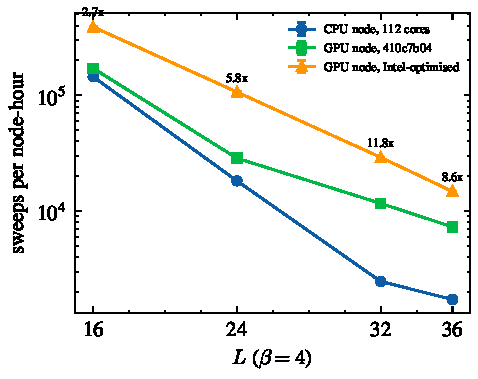
\includegraphics[width=0.6\textwidth]{throughput_vs_L}
\caption{Node throughput of the best layout per side against $L$; the factor is best GPU / best CPU.}
\end{figure}
\begin{figure}[H]\centering
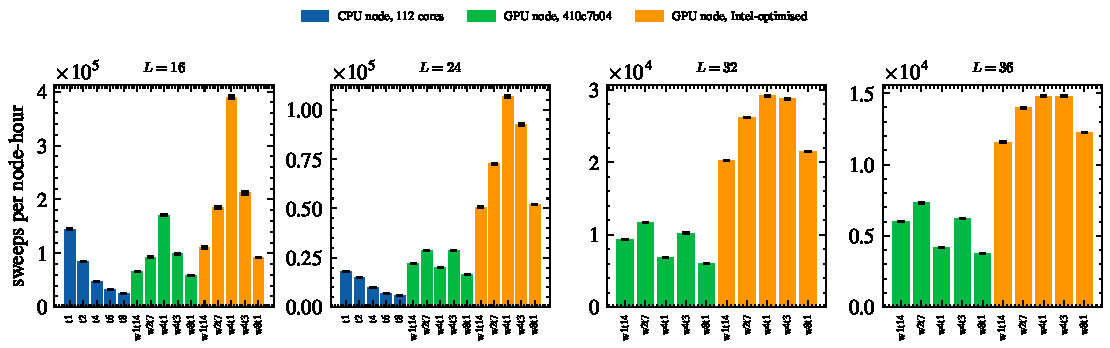
\includegraphics[width=\textwidth]{layout_scan}
\caption{Throughput of every layout (tags as in Tables 1 and 2), one panel per $L$.}
\end{figure}
\begin{figure}[H]\centering
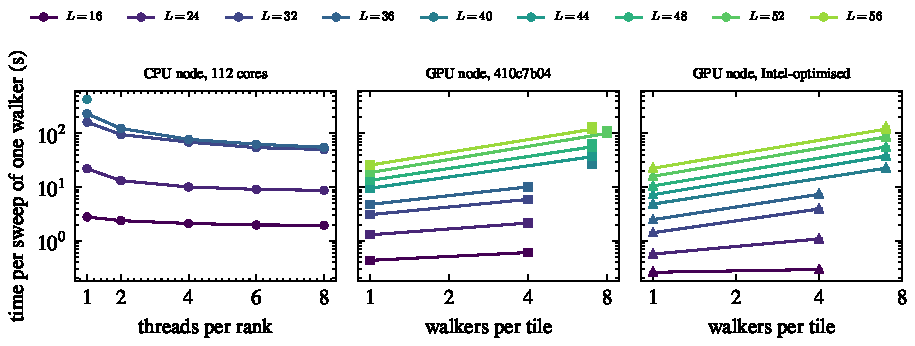
\includegraphics[width=\textwidth]{walker_time}
\caption{Time per sweep of one walker; one panel per side (CPU: against threads per rank, GPU: against walkers per tile), colour = $L$.}
\end{figure}
\begin{figure}[H]\centering
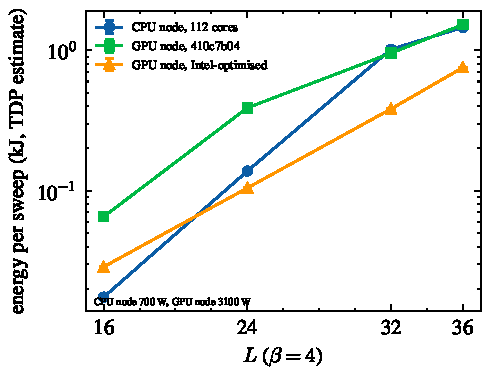
\includegraphics[width=0.6\textwidth]{energy_per_sweep}
\caption{Estimated energy per sweep of the best layout per side.}
\end{figure}
\begin{figure}[H]\centering
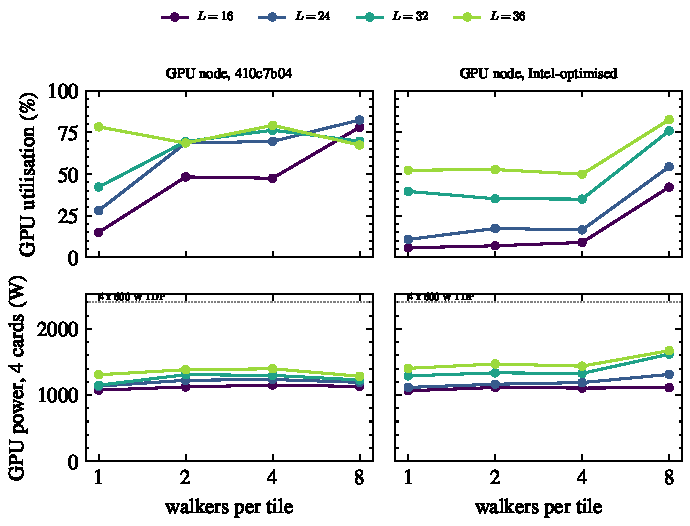
\includegraphics[width=0.7\textwidth]{gpu_usage}
\caption{Mean GPU utilisation (top) and power of the four cards (bottom), xpu-smi 1\,s samples, against walkers per tile; one column per GPU binary, colour = $L$.}
\end{figure}

\section{Extrapolation of the CPU node to larger $L$}
The CPU node was measured up to $L=40$. The cost of one sweep scales as $N^3\,N_t$ with $N=L^2$ (matrix products, QR and LU decompositions of dimension $N$) and $N_t$ time slices, so the throughput of the CPU node was fitted with $A\,L^{-6}$ (amplitude by least squares in log space) and extended to $L=56$. The free fit exponent of the measured points is given in the legend. Speedups in brackets are GPU throughput divided by the fitted CPU throughput, \emph{not measured}.
\begin{figure}[H]\centering
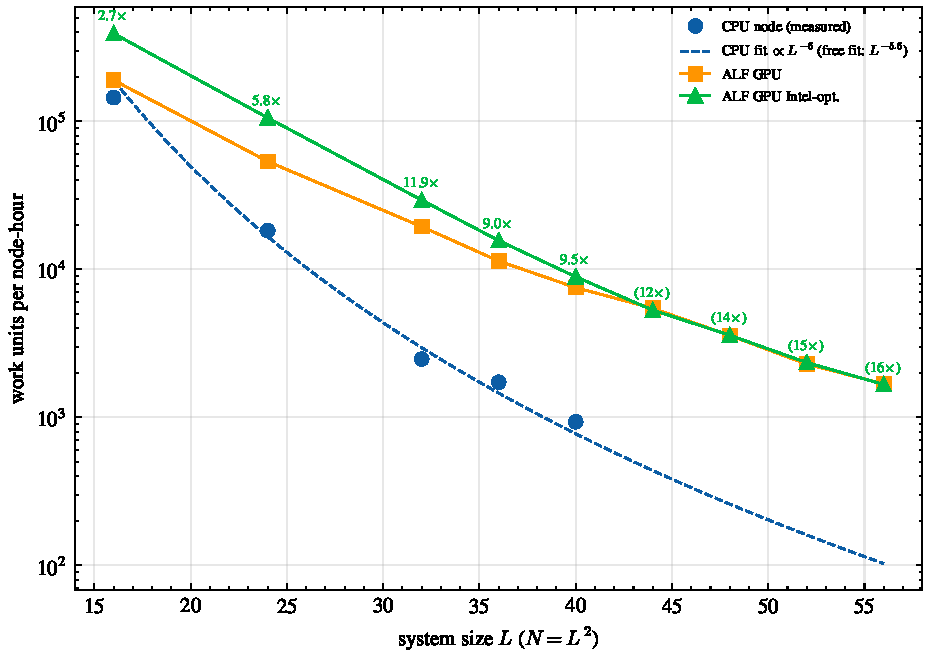
\includegraphics[width=0.75\textwidth]{cpu_fit}
\caption{CPU node: measurements and fit $\propto L^{-6}$ extended to $L=56$; GPU node curves (tuned); speedup of the Intel-optimised code over the CPU node (in brackets: extrapolated).}
\end{figure}
\begin{table}[H]\centering\small
\caption{Throughput (work units per node-hour) and speedup over the CPU node; for $L>40$ the CPU value is the fit.}
\newcommand{\FitTable}{%
\begin{tabular}{rrrrrr}
$L$ & CPU node & Intel-opt. GPU & speedup & ALF GPU speedup & CPU\\
\hline
16 & 144\,581 & 391\,560 & 2.7$\times$ & 1.3$\times$ & measured\\
24 & 18\,266 & 105\,468 & 5.8$\times$ & 2.9$\times$ & measured\\
32 & 2\,475 & 29\,338 & 11.9$\times$ & 7.8$\times$ & measured\\
36 & 1\,728 & 15\,636 & 9.0$\times$ & 6.6$\times$ & measured\\
40 & 933 & 8\,899 & 9.5$\times$ & 8.1$\times$ & measured\\
44 & 438 & 5\,304 & (12)$\times$ & (12)$\times$ & fit\\
48 & 260 & 3\,588 & (14)$\times$ & (14)$\times$ & fit\\
52 & 161 & 2\,345 & (15)$\times$ & (14)$\times$ & fit\\
56 & 103 & 1\,667 & (16)$\times$ & (16)$\times$ & fit\\
\end{tabular}}

\FitTable
\end{table}
\end{document}
